\noindent Having demonstrated that there is a negative correlation between $\mu_{rel}$ and $L$/D$_{H}$ in Figure \ref{RelativeApparentViscosityVSDistanceRatio}, $L$/D$_{H}$ could be an additional contributing factor on apparent viscosity apart from the known effects of  D$_{H}$ and H$_{D}$ on apparent viscosity. It is well-known that the apparent viscosity in micro-vessels are dominated by the thickness of the cell-free layer (CFL) and a certain length is required in order for the CFL to fully develop in a branch. This means the relative thickness of CFL to branch diameter increases with branch length which will affect the apparent viscosity of blood in the branch. So, the degree to which the CFL is recovered after a bifurcating point should greatly affect the apparent viscosity in the downstream branch. \\

\noindent A closer look at the distribution of $L$ against D$_{H}$ (see Figure \ref{BranchLengthVSBranchDiamete}) shows a negative correlation between $L$ and D$_{H}$ was observed where the branch length decreases with branch diameter. Given that the context of "longer" and "shorter" is a relative comparison between the two child branches in each bifurcation, the majority of the longer child branches were found to have smaller diameters while shorter branches have larger diameters. To evaluate the potential of a negative correlation, the Pearson correlation coefficient (r) was calculated to measure the ratio of the covariance of branch diameter and branch length to the product of their standard deviations. This gives us the measure of the linear relationship between these two parameters. From Figure \ref{BranchLengthVSBranchDiamete}, the value r $=$ -0.535 indicates a strong negative correlation (0.5 $<$ $\lvert$ r $\rvert$ $<$ 1) between the length and diameter of vessels within the studied networks. Furthermore, a p-value $<$ 0.001 was calculated which suggests that the results obtained were statistically highly significant and are less than 1 in 1000 chance of being wrong. Therefore, it is apparent that the negative correlation does clearly exist within the studied networks. 


\begin{figure}[H]
\centering
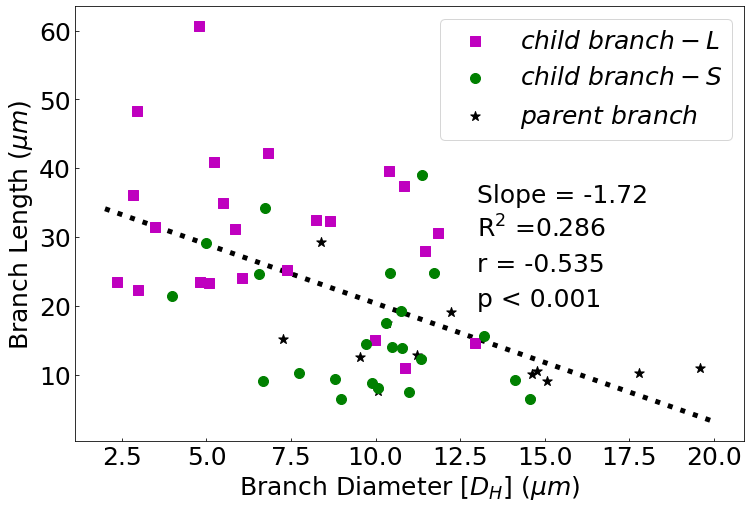
\includegraphics[width=0.8\textwidth]{images/BranchLengthVSBranchDiameter.png}
\caption{\textit{Distribution of branch length against branch diameter with best-fitted line. The "L"/"S" indicate the relatively longer (purple squares) and shorter (green circles) child branches in each diverging bifurcation respectively.} \label{BranchLengthVSBranchDiamete}}
\end{figure}

\noindent Considering that the branches from simulation data have limited branch length, most of the CFLs are not fully developed in the branches across all of the ROIs. The lack of symmetrical CFL recovery could be due to the migration of RBCs induced by boundary interactions where the RBCs tend to migrate away from the solid boundaries (i.e. vessel walls) when suspended in a shear flow. Therefore, the lack of CFL recovery and insufficient RBC migration due to limited interbifurcation distances (i.e. $L$/D$_{H}$ for the branch between bifurcations) are the causes for the deviation between simulation data and empirical predictions from Pries Viscosity Models (\textit{in-vivo} and \textit{in-vitro}). In other words, the smaller the $L$/D$_{H}$, the more underdeveloped the CFL in the downstream branch will be and hence, the cross-sectional distribution of RBCs is disturbed after the bifurcation and will require a certain distance (i.e. $L$/D$_{H}$) to recover back to its original shape of the haematocrit profile. 